\documentclass[aspectratio=169,11pt]{beamer}
\usetheme{default}
\usecolortheme{dove}
\setbeamertemplate{navigation symbols}{}
\setbeamertemplate{footline}[frame number]
\usepackage[T1]{fontenc}
\usepackage{lmodern}
\usepackage{amsmath,amssymb}
\usepackage{listings}
\usepackage{tikz}
\usetikzlibrary{arrows.meta,positioning,shapes.misc,fit,calc}
\usepackage{booktabs}
\usepackage{array}

\definecolor{acc}{HTML}{1F5FAD}
\definecolor{new}{HTML}{B4421C}
\definecolor{keep}{HTML}{2E7D32}
\setbeamercolor{frametitle}{fg=acc}
\setbeamercolor{structure}{fg=acc}

\lstset{basicstyle=\ttfamily\scriptsize, columns=fullflexible, keepspaces=true,
  keywordstyle=\color{acc}\bfseries, commentstyle=\color{gray}, showstringspaces=false,
  morekeywords={\#amosum,\#jointsum,\#jointcap,\#sum}, morecomment=[l]{\%}, escapechar=`}

\newcommand{\file}[1]{{\small\texttt{\color{acc}#1}}}
\newcommand{\NEW}{\textcolor{new}{\textbf{new}}}
\newcommand{\GEN}{\textcolor{keep}{\textbf{generalised}}}

\title{From \texttt{\#amosum} to \texttt{\#jointsum}}
\subtitle{The amoclingo pipeline, and how a knapsack-aware sum fits into it}
\date{16 November 2026 --- branch \texttt{jointsum}}

\begin{document}

\begin{frame}
  \titlepage
  \centering\footnotesize
  Part I: how \texttt{amoclingo} works today (code outside \texttt{ijcai\_version}).\\
  Part II: the motivating example.\quad
  Part III: \texttt{\#jointsum}, the hull, and where it plugs in.\quad
  Part IV: \texttt{\#jointsum} vs plain LP (and how LP is solved).\quad Part V: decisions.
\end{frame}

%=====================================================================
\section{Part I --- the amosum pipeline}

\begin{frame}{The big picture}
\centering
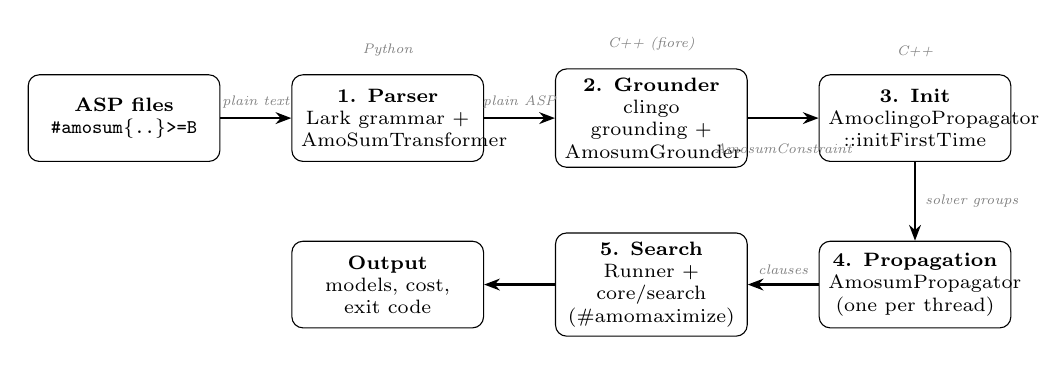
\begin{tikzpicture}[node distance=4mm and 9mm,
  box/.style={draw, rounded corners, align=center, font=\scriptsize, minimum height=11mm, text width=22mm, fill=white},
  lang/.style={font=\tiny\itshape, text=gray},
  arr/.style={-{Stealth[length=2mm]}, thick}]
  \node[box] (in) {\textbf{ASP files}\\\texttt{\#amosum\{..\}>=B}};
  \node[box, right=of in] (par) {\textbf{1. Parser}\\Lark grammar +\\AmoSumTransformer};
  \node[box, right=of par] (gr) {\textbf{2. Grounder}\\clingo grounding +\\AmosumGrounder};
  \node[box, right=of gr] (ini) {\textbf{3. Init}\\AmoclingoPropagator\\::initFirstTime};
  \node[box, below=10mm of ini] (prop) {\textbf{4. Propagation}\\AmosumPropagator\\(one per thread)};
  \node[box, left=of prop] (search) {\textbf{5. Search}\\Runner + core/search\\(\#amomaximize)};
  \node[box, left=of search] (out) {\textbf{Output}\\models, cost,\\exit code};
  \draw[arr] (in) -- node[above,lang]{plain text} (par);
  \draw[arr] (par) -- node[above,lang]{plain ASP} (gr);
  \draw[arr] (gr) -- node[below=2mm,lang]{AmosumConstraint} (ini);
  \draw[arr] (ini) -- node[right,lang]{solver groups} (prop);
  \draw[arr] (prop) -- node[above,lang]{clauses} (search);
  \draw[arr] (search) -- (out);
  \node[lang, above=1mm of par] {Python};
  \node[lang, above=1mm of gr] {C++ (fiore)};
  \node[lang, above=1mm of ini] {C++};
\end{tikzpicture}

\vspace{4mm}
\footnotesize
\texttt{amoclingo enc.asp inst.asp [--reason ..] [--lazy ..] [--opt-strategy ..]} is a Python wrapper
(\file{amosum/amoclingo/\_\_main\_\_.py}): it rewrites each file into a temporary one, then runs
\file{cpp/bin/amoclingo-core [options] rewritten-files}. \texttt{-lg py} runs the Python mirror instead, and
\texttt{amowasp} feeds the same rewritten program to WASP.
\end{frame}

\begin{frame}[fragile]{Step 1 --- the parser: \texttt{\#amosum} becomes plain ASP}
\footnotesize
\file{amosum/amosumparser/}: \texttt{AmoSumGrammar.py} (ASP-Core + \texttt{amosum\_rule}),
\texttt{AmoSumTransformer.py} (rewriting), \texttt{rewrite.py} (on files). Real output:
\begin{columns}[T]
\begin{column}{.42\textwidth}
\textbf{Input}
\begin{lstlisting}
#amosum{ V*VAL,X : in(X,V),
          object(X,_,VAL) [X] } >= 20.
\end{lstlisting}
\textbf{Element} = \textit{tuple} \texttt{V*VAL,X}, \textit{condition}, \textit{group} \texttt{[X]}.\\[1mm]
Semantics: at most one element per group is true (AMO), and the sum of the true weights is $\ge 20$.
\end{column}
\begin{column}{.56\textwidth}
\textbf{Output (\texttt{python -O -m amosum.amosumparser})}
\begin{lstlisting}
__element__((0),(V*VAL,X),(X)) :-
        in(X,V), object(X,_,VAL).
{__group__(__element__((0),(V*VAL,X),(X)),
           "+", V*VAL, (X), (0))} :-
        in(X,V), object(X,_,VAL).
__lb__(20,(0)).
__aux__((0), ge_amo).
{__group__(__aux__((0),ge_amo), "-", 20,
           (__aux__((0),ge_amo)), (0))}.
\end{lstlisting}
\end{column}
\end{columns}
\vspace{1mm}
\begin{itemize}\setlength\itemsep{0pt}
\item \texttt{\_\_group\_\_(Lit, Sign, W, G, ID)} only \emph{describes} the constraint: its atoms are later forced false.
\item \texttt{\_\_lb\_\_}/\texttt{\_\_ub\_\_} give the bound and the direction; \texttt{\_\_aux\_\_} gives the type
  (\texttt{ge\_amo}, \texttt{ge\_eo}, \texttt{le\_amo}, \texttt{le\_eo}, \texttt{amomaximize}).
\item The ID is \texttt{(counter, body without built-ins)}: one constraint per ground body.
\end{itemize}
\end{frame}

\begin{frame}{Step 2 --- grounding and reading the constraint back}
\footnotesize
\file{amosum/core/cpp/program.cpp}: \texttt{AmosumProgram::AmosumGrounder::ground}
\begin{enumerate}\setlength\itemsep{2pt}
\item fiore grounds the rewritten program with clingo (\texttt{fiore::Program::ProgramGrounder}).
\item It scans the ground atoms: each \texttt{\_\_group\_\_/5} adds a \texttt{GroupElement} (literal, weight, group, tuple, aux)
  to \texttt{AggregateData[ID]}. \texttt{\_\_lb\_\_}/\texttt{\_\_ub\_\_} set the bound and \texttt{ge}, and \texttt{\_\_aux\_\_} sets the type.
\item \textbf{normalize} (program level, set semantics):
  \begin{itemize}\setlength\itemsep{0pt}
  \item a tuple in several groups $\Rightarrow$ fresh OR atom \texttt{\_\_tuple\_\_} of weight $w$ in its own group;
    the original elements stay with weight 0 (``moved'' literals);
  \item equal weights inside one group $\Rightarrow$ one OR atom \texttt{\_\_same\_\_} (valid only because the group is AMO).
  \end{itemize}
\item One \texttt{AmosumConstraint} (a \texttt{fiore::PBConstraint}) per aggregate: \texttt{id, type, ge, bound, groups,
  weight function}. \texttt{\#amomaximize} is kept apart as \texttt{amomaximizeConstraint}.
\end{enumerate}
\vspace{1mm}
\file{amosum/amoclingo/cpp/solver.cpp}: \texttt{AmosumClingoSolver::init} registers
\textbf{one \texttt{AmoclingoPropagator} per constraint} with clingo.
\end{frame}

\begin{frame}{Step 3 --- initialisation over solver literals}
\footnotesize
\file{amosum/amoclingo/cpp/propagator.cpp}: \texttt{AmoclingoPropagator::initFirstTime}
(a \texttt{fiore::PropagatorPBConstraint}, i.e.\ the clingo glue)
\begin{enumerate}\setlength\itemsep{2pt}
\item \texttt{buildSolvingGroups} (\file{core/cpp/propagator.cpp}): program literals $\to$ solver literals.
  It handles literals fixed to TOP/BOTTOM, merges equal solver literals and orders each group by \emph{(weight, literal)}.
  The result is \texttt{AmosumSolvingGroups}, \textbf{shared read-only} by all threads.
\item It adds watches (both polarities, except for \texttt{le\_amo}).
\item It creates one \texttt{AmosumPropagator} \emph{implementation} per solver thread.
\item The \texttt{\_\_group\_\_} atoms are forced false (unit clauses).
\end{enumerate}
\vspace{2mm}
\begin{block}{Per-thread state (\texttt{AmosumThreadGroup})}
\texttt{ordL} (literals by weight), \texttt{maxUndI}/\texttt{minUndI} (max/min undefined), \texttt{countUndef},
\texttt{trueLiteral}, plus the moved literals. Globally: \texttt{mpsValue} = max (ge) / min (le) possible sum,
\texttt{currentSum}, \texttt{reasons[lit]}, \texttt{slack[lit]}.
\end{block}
\end{frame}

\begin{frame}{Step 4 --- one propagation round (fiore's template)}
\footnotesize
\begin{columns}[T]
\begin{column}{.5\textwidth}
\textbf{\texttt{updatePhase(changes)}}
\begin{itemize}\setlength\itemsep{1pt}
\item for each literal $c$ that became true:\\
  \texttt{onMemberTrue} / \texttt{onMemberFalse} / moved;
\item update the group's \texttt{contribution}:\\
  $\text{mps} \mathrel{+}= \text{after} - \text{before}$;
\item if mps $<$ lb (ge) $\Rightarrow$ \textbf{conflict},\\
  explained by \texttt{explainMaxOfGroups};
\item \texttt{nextPhase} = changed $\wedge$ lazy condition.
\end{itemize}
\textbf{\texttt{onLiteralsUndefined}} (undo) reverses the updates.
\end{column}
\begin{column}{.5\textwidth}
\textbf{\texttt{propagatePhase}} $\to$ \texttt{propagateGeAmo}, for each undecided group $g$:
\begin{itemize}\setlength\itemsep{1pt}
\item $\text{base} = \text{mps} - \text{contrib}(g)$;
\item if $\text{base} + w(\text{2nd max}) < \text{lb}$: \textbf{max literal must be true};
\item for $l$ by increasing weight: if $\text{base} + w(l) < \text{lb}$: \textbf{$\neg l$}, else stop.
\end{itemize}
Reasons:
\begin{itemize}\setlength\itemsep{1pt}
\item \texttt{explainMaxOfGroups}: in the other groups, the false literals heavier than the current max, or the true literal;
\item \texttt{--reason min/minfly}: leave out what the slack $\text{lb}-\text{mps}_h$ allows (the greedy increments).
\end{itemize}
\end{column}
\end{columns}
\vspace{1mm}
fiore turns each derived literal and its reason into a clause (\texttt{addClause}) and calls clingo's propagate.
\end{frame}

\begin{frame}{Step 5 --- search and output}
\footnotesize
\begin{itemize}
\item \file{amoclingo/cpp/runner.cpp}: plain satisfiability, or optimisation of a single \texttt{\#amomaximize}.
\item \file{core/cpp/search/}: \texttt{sat-unsat}, \texttt{unsat-sat}, \texttt{binary}, \texttt{progression}. Each is
  a sequence of solve calls in which \texttt{AmosumClingoBackend::setBound} changes the constraint's bound \emph{live}.
  The propagator notices it (\texttt{lastBound}) and propagates again.
\item \texttt{AmosumClingoAssignment} prints models (\texttt{Amomaximize Cost:} \dots).
  Exit codes: 10 SAT, 20 UNSAT, 30 OPTIMUM, \dots
\end{itemize}
\vspace{3mm}
\begin{block}{Mirrors and rules to keep in mind}
\begin{itemize}\setlength\itemsep{0pt}
\item C++ $\leftrightarrow$ Python file by file (\texttt{cpp/x.cpp} $\leftrightarrow$ \texttt{py/x.py}); WASP is Python only.
\item \texttt{amosum/ijcai\_version/} is frozen.
\item Tests: \texttt{tests/unit/\{cpp,python\}}, \texttt{tests/correctness/check\_correctness.py} (against clingo),
  light benchmarks \texttt{ga gc kn kn\_toy}.
\end{itemize}
\end{block}
\end{frame}

%=====================================================================
\section{Part II --- motivating example}

\begin{frame}{Why amosum is not enough}
\footnotesize
\begin{columns}[T]
\begin{column}{.48\textwidth}
\textbf{Toy example}
\[
(1)\; 5a + 2b + 3c \ge 5 \qquad (2)\; 2b + c \le 2
\]
\begin{itemize}\setlength\itemsep{1pt}
\item Alone, (1) has mps $= 10 \ge 5$, so nothing is propagated.
\item With (2), $\{b,c\}$ is worth at most 3 (integer) or 4 (LP), so $\neg a \Rightarrow \le 4 < 5$, hence \textbf{$a$ must be true}.
\item amosum is the case where (2) is $b + c \le 1$ (costs 1, capacity 1).
\end{itemize}
\end{column}
\begin{column}{.5\textwidth}
\textbf{Knapsack UNSAT (metaprop benchmark)}\\[1mm]
value $\ge$ MIN with weight $\le$ CAP, 20 copies per item, encoded as AMO over \texttt{in\_knapsack(X,V)}.
\begin{itemize}\setlength\itemsep{1pt}
\item \texttt{\#amosum} sees only the value constraint: mps is huge.
\item The LP of both constraints is below MIN:\\
  0056: $864\,044 < 914\,194$\\
  0096: $1\,273\,508 < 1\,429\,327$.
\item CP-SAT proves these instantly; clingo and amoclingo don't.
\end{itemize}
\end{column}
\end{columns}
\end{frame}

\begin{frame}{Option 3, step 1: a tiny knapsack}
\footnotesize
\begin{columns}[T]
\begin{column}{.45\textwidth}
\begin{center}
\begin{tabular}{crrr}\toprule
item & weight $w$ & value $p$ & ratio $p/w$\\\midrule
1 & 2 & 8 & 4\\
2 & 3 & 9 & 3\\
3 & 4 & 8 & 2\\
4 & 5 & 5 & 1\\\bottomrule
\end{tabular}
\end{center}
\[
\begin{aligned}
(V)&\quad 8x_1 + 9x_2 + 8x_3 + 5x_4 \;\ge\; 22 \quad\text{(value)}\\
(W)&\quad 2x_1 + 3x_2 + 4x_3 + 5x_4 \;\le\; 7 \quad\text{(capacity)}
\end{aligned}
\]
\end{column}
\begin{column}{.52\textwidth}
\begin{itemize}\setlength\itemsep{3pt}
\item $(V)$ alone is easy to satisfy: take everything, $30 \ge 22$.
\item $(W)$ alone is easy too: take nothing.
\item \textbf{Together}: the best value within capacity 7 is $17$ (items 1+2, or 2+3), so the problem is \textbf{UNSAT}.
\item A propagator that looks at $(V)$ alone (like \texttt{\#sum} or \texttt{\#amosum}) only sees ``mps $= 30 \ge 22$'', and the
  solver has to enumerate to find the conflict.
\end{itemize}
\vspace{2mm}
\textbf{Goal}: a \emph{cheap} certificate that $(V)\wedge(W)$ is impossible, without solving the integer problem.
\end{column}
\end{columns}
\end{frame}

\begin{frame}{Option 3, step 2: the Dantzig bound (greedy by ratio)}
\footnotesize
\textbf{Relax}: allow fractions $x_i \in [0,1]$ (the LP). Then the best filling is greedy: sort the items by \textbf{value per unit
of capacity} ($p/w$) and fill the knapsack from the best; the first item that does not fit (the \textbf{critical item})
is taken \emph{partially}.
\vspace{1mm}
\begin{center}
\begin{tabular}{clccc}\toprule
step & item (ratio) & take & capacity left & value so far\\\midrule
1 & item 1 ($r{=}4$) & all ($w{=}2$) & $7-2 = 5$ & 8\\
2 & item 2 ($r{=}3$) & all ($w{=}3$) & $5-3 = 2$ & 17\\
3 & \textbf{item 3 ($r{=}2$), critical} & $\frac{2}{4}$ of it & 0 & $17 + \frac24\cdot 8 = \mathbf{21}$\\
4 & item 4 ($r{=}1$) & nothing & 0 & 21\\\bottomrule
\end{tabular}
\end{center}
\begin{itemize}\setlength\itemsep{2pt}
\item \textbf{Why greedy is optimal for the LP}: one unit of capacity is worth $4$ in item 1, $3$ in item 2, \dots;
  moving capacity from a worse ratio to a better one never loses value.
\item The LP optimum is an \textbf{upper bound} on every integer solution: $17 \le 21$.
\item $21 < 22$ $\Rightarrow$ $(V)\wedge(W)$ is \textbf{UNSAT}, proven without any search.
\end{itemize}
\textbf{But} clingo has no LP inside. Can we write this argument as \emph{one} ordinary \texttt{\#sum}? $\to$ Lagrange.
\end{frame}

\begin{frame}{Option 3, step 3: merging two constraints into one (Lagrangian)}
\footnotesize
Pick a \textbf{price} $\lambda \ge 0$ for one unit of capacity. Every solution satisfies both
\[
\sum_i p_i x_i \ge K \qquad\text{and}\qquad \lambda\Big(C - \sum_i w_i x_i\Big) \ge 0 \quad(\text{since } \lambda\ge0).
\]
\textbf{Add them}:
\[
\boxed{\;\sum_i (p_i - \lambda w_i)\,x_i \;\ge\; K - \lambda C\;}
\]
This is \textbf{implied} by $(V)\wedge(W)$, so adding it to the program never removes a solution (\textbf{sound} for every $\lambda\ge 0$).
\vspace{1mm}
\begin{columns}[T]
\begin{column}{.5\textwidth}
\textbf{Example} with $\lambda = 2$ ($K{=}22$, $C{=}7$):
\[
4x_1 + 3x_2 + 0x_3 - 5x_4 \;\ge\; 22 - 14 = 8.
\]
\end{column}
\begin{column}{.48\textwidth}
\textbf{Checking it is trivial}: its largest possible left side takes exactly the positive coefficients:
$4 + 3 + 0 = 7 < 8$.\\[1mm]
$\Rightarrow$ the merged constraint alone is violated, \textbf{UNSAT}.
\end{column}
\end{columns}
\vspace{2mm}
Any \texttt{\#sum} propagator does this check at the root: it is exactly ``mps $<$ bound''.
\end{frame}

\begin{frame}{Option 3, step 4: which price $\lambda$?}
\footnotesize
\begin{columns}[T]
\begin{column}{.5\textwidth}
For each $\lambda$, the merged constraint fails iff
\(
L(\lambda) = \lambda C + \sum_i \max(0,\ p_i - \lambda w_i) < K .
\)\\[1mm]
$L(\lambda)$ is an \textbf{upper bound on the best value} for every $\lambda\ge0$.
\begin{center}\scriptsize\renewcommand{\arraystretch}{0.95}
\begin{tabular}{crrcc}\toprule
$\lambda$ & $\lambda C$ & $\sum\max(0,\cdot)$ & $L(\lambda)$ & $< 22$?\\\midrule
0 & 0 & 30 & 30 & no\\
1 & 7 & 6+6+4+0 = 16 & 23 & no\\
\textbf{2} & 14 & 4+3+0 = 7 & \textbf{21} & \textbf{yes}\\
3 & 21 & 2+0 = 2 & 23 & no\\
4 & 28 & 0 & 28 & no\\\bottomrule
\end{tabular}
\end{center}
\end{column}
\begin{column}{.48\textwidth}
\centering
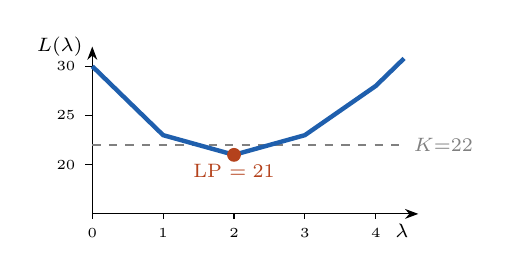
\begin{tikzpicture}[x=9mm,y=1.25mm]
  \draw[-{Stealth}] (0,15) -- (4.6,15) node[below left]{\scriptsize $\lambda$};
  \draw[-{Stealth}] (0,15) -- (0,32) node[left]{\scriptsize $L(\lambda)$};
  \foreach \x in {0,...,4} \draw (\x,15) -- (\x,14.5) node[below]{\tiny\x};
  \foreach \y in {20,25,30} \draw (0,\y) -- (-0.1,\y) node[left]{\tiny\y};
  \draw[dashed, gray] (0,22) -- (4.4,22) node[right]{\scriptsize $K{=}22$};
  \draw[ultra thick, acc] (0,30) -- (1,23) -- (2,21) -- (3,23) -- (4,28) -- (4.4,30.8);
  \fill[new] (2,21) circle (2.5pt) node[below]{\scriptsize LP $=21$};
\end{tikzpicture}
\end{column}
\end{columns}
\scriptsize
\begin{itemize}\setlength\itemsep{1pt}
\item $L$ is piecewise linear and convex, with breakpoints at the ratios $4,3,2,1$.
\item Its minimum is at $\lambda = 2$ = \textbf{the ratio of the critical item}, and the minimum value $21$ \textbf{equals the Dantzig
  bound} (LP duality). So: run Dantzig once, read $\lambda = r_c$ off the critical item, giving the strongest merged constraint.
\item Why the critical ratio: the slope of $L$ is $C - \sum_{r_i > \lambda} w_i$, which turns from negative to positive exactly
  when the items better than $\lambda$ stop fitting.
\end{itemize}
\end{frame}

\begin{frame}[fragile]{Option 3, step 5: from the toy to the benchmark}
\footnotesize
\textbf{Integers}: $\lambda = r_c = p_c / w_c = N/D$ is a fraction. Multiply the merged constraint by $D$:
\[
\sum_i (D\,p_i - N\,w_i)\,x_i \;\ge\; D K - N C .
\]
\textbf{Copies}: in the benchmark, item $X$ can be taken 0..20 times, via the AMO over \texttt{in\_knapsack(X,V)} ($V$ = copies,
coefficient $V\!\cdot c_X$, with $c_X = D p_X - N w_X$).
\begin{columns}[T]
\begin{column}{.5\textwidth}
\textbf{Pitfall}, with up to 3 copies and $c_X > 0$:
\begin{lstlisting}
#sum{ V*C,X,V : in_knapsack(X,V), ... }
\end{lstlisting}
\texttt{\#sum} doesn't know the AMO, so its largest left side takes $V{=}1,2,3$ together: $c+2c+3c = 6c$, not $3c$.
For 20 copies: $210c$ instead of $20c$. The bound is too weak and clingo does not refute (60\,s timeout).
\end{column}
\begin{column}{.48\textwidth}
\textbf{Fix: order encoding}: \texttt{geq(X,K)} = ``at least $K$ copies'', $K = 1..20$, each with coefficient $c_X$.
\begin{lstlisting}
geq(X,K) :- in_knapsack(X,V), K=1..V.
\end{lstlisting}
The largest left side is now $20\,c_X^{+}$ per item, the true one, so the root check is exactly $L(\lambda) < K$.
\end{column}
\end{columns}
\vspace{1mm}
\texttt{lagr.py} runs Dantzig with 20 copies per item, finds the critical item and prints \texttt{lagr(N,D)}.
\end{frame}

\begin{frame}[fragile]{Option 3, step 6: the aggregate and the results}
\footnotesize
\file{experiments/jointsum/motivating\_example/encoding-plain-amo-lagr.asp} (added to the plain encoding):
\begin{lstlisting}
geq(X,K) :- in_knapsack(X,V), K=1..V.                     % order encoding
coef(X, VALUE*D - WEIGHT*N) :- object(X,WEIGHT,VALUE), lagr(N,D).
rhs(MIN*D - CAP*N)          :- lb(MIN,1), ub(CAP,0), lagr(N,D).
:- #sum{C,X,K: geq(X,K), coef(X,C)} < R, rhs(R).           % merged constraint
\end{lstlisting}
\begin{center}
\begin{tabular}{lcrrl}\toprule
instance & $\lambda = N/D$ & $L(\lambda)$ = LP & MIN & clingo + merged constraint \\\midrule
0056 & 1629/182 & 864\,044 & 914\,194 & UNSAT, 0 choices, 1 conflict, 0.006\,s\\
0096 & 1326/162 & 1\,273\,508 & 1\,429\,327 & UNSAT, 0 choices, 1 conflict, 0.006\,s\\\bottomrule
\end{tabular}
\end{center}
\textbf{Limits}: $\lambda$ is \emph{frozen at the root}, so during search the merged constraint is weaker than the LP at that node.
It also needs the order encoding and a script per problem. \textbf{\texttt{\#jointsum} (option 2)} re-optimises $\lambda$ at every node
inside the propagator, on the natural encoding (Part III, ``Dual view'').
\end{frame}


%=====================================================================
\section{Part III --- jointsum}

\begin{frame}[fragile]{\texttt{\#jointsum}: classical sums, propagated together}
\scriptsize
\begin{columns}[T]
\begin{column}{.5\textwidth}
\textbf{Syntax}: the same as clingo's \texttt{\#sum} (set semantics, no groups).
\begin{lstlisting}
#jointsum{ W,T : cond ; ... } >= B : body.
#jointsum{ W,T : cond ; ... } <= B : body.
\end{lstlisting}
\textbf{Toy example}
\begin{lstlisting}
#jointsum{ 5,a:a ; 2,b:b ; 3,c:c } >= 5.
#jointsum{ 2,b:b ; 1,c:c } <= 2.
\end{lstlisting}
\textbf{Knapsack, natural encoding}
\begin{lstlisting}
#jointsum{ V*VAL,X : in_knapsack(X,V),
           object(X,_,VAL) } >= MIN : lb(MIN,1).
#jointsum{ V*W,X : in_knapsack(X,V),
           object(X,W,_) } <= CAP : ub(CAP,0).
% AMO of item X
#jointsum{ 1,X,V : in_knapsack(X,V) } <= 1
           : object(X,_,_).
\end{lstlisting}
\end{column}
\begin{column}{.48\textwidth}
\textbf{Only \texttt{\#jointsum} statements} take part, and \textbf{every statement is both a target and a side constraint}
of the others (next slide). For a target $\ge K$, the statements that bound it from above are:
\begin{itemize}\setlength\itemsep{1pt}
\item an \textbf{AMO} (all weights 1, $\le 1$), which gives a \textbf{class};
\item any other $\le k$, which gives a \textbf{capacity group};
\item classes inside a capacity group are \textbf{nested} in it;
\item a literal in none of them is a one-option class with no capacity, so its bound is just $w$.
\end{itemize}
\vspace{1mm}
A side literal outside the target (weight 0 there) still uses capacity when true.\\[1mm]
v1: if two side constraints overlap without nesting, each literal goes to the one with the best bound (weight splitting comes later).
\end{column}
\end{columns}
\end{frame}

\begin{frame}{Every statement is a target \emph{and} a side constraint}
\scriptsize
Each \texttt{\#jointsum} statement gets its own propagator (it is a target), and it restricts the space of every other
statement it shares literals with (it is a side constraint). The \textbf{direction} only decides \emph{how} it enters a bound:
\begin{center}
\begin{tabular}{>{\raggedright\arraybackslash}p{34mm}>{\raggedright\arraybackslash}p{52mm}>{\raggedright\arraybackslash}p{52mm}}\toprule
target & bounded by the $\le$ statements & bounded by the $\ge$ statements\\\midrule
$\ge K$: needs an \textbf{upper} bound (max possible sum)
  & they \textbf{cap} it: capacity groups, AMO classes, \textbf{upper} hull
  & the ``at least'' part: an EO class must pick an option, so it pays its cheapest cost\\
$\le K$: needs a \textbf{lower} bound (min possible sum)
  & the ``at most'' part (mirror of the left cell)
  & they \textbf{force} it: covering groups, at-least-one classes, \textbf{lower} hull\\\bottomrule
\end{tabular}
\end{center}
The two rows are mirror images (negate the weights: $\sum w x \le K \iff \sum (-w) x \ge -K$), so \texttt{<=} and \texttt{>=}
come in the same release, with the same code.
\vspace{1mm}
\begin{block}{A same-direction statement matters too}
$5a \ge 5$,\ \ $a + b \le 1$,\ \ $b \ge 1$. The propagator of $b \ge 1$ derives $b$; then $a+b\le 1$ (as a target) derives $\neg a$;
then $5a \ge 5$ fails. So statements already \textbf{cooperate through propagation}, on assigned literals.
The joint \emph{bound} adds LP reasoning on the \emph{undefined} ones. v1 uses the greedy (hull + Dantzig), which is exact for
one resource per group plus its classes; a group restricted by $\le$ \emph{and} $\ge$ statements at once is a general LP (no
greedy), so that is future work.
\end{block}
\end{frame}

\begin{frame}{Knapsack: which side constraint owns \texttt{in\_knapsack(X,V)}?}
\footnotesize
Item $X$ (weight $w$, value \textit{val}) has 20 literals $x_1,\dots,x_{20}$. Option $x_V$ = ``take $V$ copies'', with
cost $V w$ and value $V\cdot\textit{val}$. Each $x_V$ is in \textbf{two} side constraints: the capacity and the AMO of $X$.
\vspace{2mm}
\begin{center}
\begin{tabular}{p{38mm}p{62mm}r}\toprule
grouping & what the bound sees & bound on 0096\\\midrule
(a) group = AMO of $X$ & amosum: $UB_X = 20\cdot\textit{val}$; the capacity is ignored & huge\\
(b) group = capacity, flat & $x_1..x_{20}$ as independent items: $1{+}\dots{+}20 = 210$ copies; the AMO is ignored & $1\,821\,737$\\
(c) \textbf{capacity group with AMO classes} & multiple-choice knapsack: $\le 1$ option per class, within the capacity & $\mathbf{1\,273\,508}$\\\bottomrule
\end{tabular}
\end{center}
\vspace{2mm}
MIN $= 1\,429\,327$: only (c) is below MIN, so only (c) proves the instance UNSAT. It is the LP of the whole problem.\\[2mm]
The next slides explain how to compute the bound of (c): the \textbf{upper convex hull} of each class.
\end{frame}

\begin{frame}{The multiple-choice knapsack (MCKP) and its LP}
\footnotesize
One \textbf{group} = one capacity $R$ (what is left of $k$), plus \textbf{classes} $C_1, C_2, \dots$\\
Each class is a set of \textbf{options} $i$ with cost $c_i$ and value $p_i$, and at most one option per class may be true (AMO).
\[
\textbf{integer:}\quad \max \sum_{C}\sum_{i \in C} p_i x_i \quad\text{s.t.}\quad \sum_C\sum_{i\in C} c_i x_i \le R,\quad
\sum_{i \in C} x_i \le 1,\quad x_i \in \{0,1\}.
\]
\textbf{LP relaxation}: $x_i \in [0,1]$. Look at a single class: it now picks \emph{fractions} $\lambda_i \ge 0$ with
$\sum_i \lambda_i \le 1$, and contributes
\[
(\text{cost}, \text{value}) \;=\; \Big(\sum_i \lambda_i c_i,\; \sum_i \lambda_i p_i\Big).
\]
Because $\sum\lambda_i \le 1$, the missing part $1 - \sum\lambda_i$ is the option ``take nothing'' $= (0,0)$.
So the pairs a class can reach are exactly the \textbf{convex combinations} of its points
\[
\{(0,0)\} \cup \{(c_i, p_i) : i \in C\},
\]
i.e.\ the \textbf{convex hull} of these points: the smallest convex polygon that contains them all
(think of a rubber band stretched around the points).
\vspace{1mm}
\begin{block}{Question for the LP}
If the class may spend a budget $b$ of capacity, what is the \emph{best} value it can reach?\quad
$f_C(b) = \max\{\,\text{value} : (\text{cost},\text{value}) \in \text{hull},\ \text{cost} \le b\,\}$.
\end{block}
\end{frame}

\begin{frame}{What is the hull? A worked class}
\footnotesize
\begin{columns}[T]
\begin{column}{.5\textwidth}
\centering
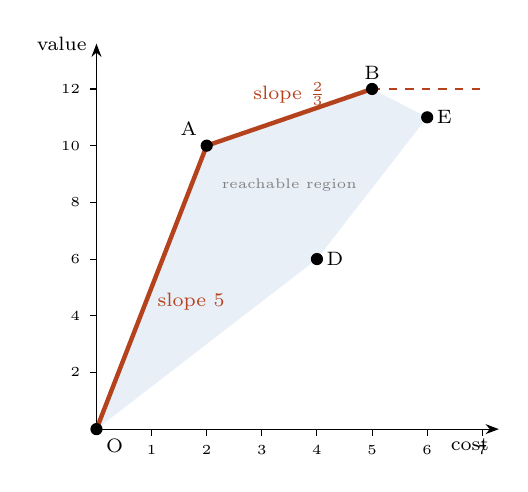
\begin{tikzpicture}[x=7mm,y=3.6mm]
  \fill[acc!10] (0,0) -- (4,6) -- (6,11) -- (5,12) -- (2,10) -- cycle;
  \draw[-{Stealth}] (0,0) -- (7.3,0) node[below left]{\scriptsize cost};
  \draw[-{Stealth}] (0,0) -- (0,13.6) node[left]{\scriptsize value};
  \foreach \x in {1,...,7} \draw (\x,0) -- (\x,-0.25) node[below]{\tiny\x};
  \foreach \y in {2,4,...,12} \draw (0,\y) -- (-0.12,\y) node[left]{\tiny\y};
  \draw[ultra thick, new] (0,0) -- node[right, pos=.45]{\scriptsize slope 5} (2,10) -- node[above, pos=.5]{\scriptsize slope $\frac23$} (5,12);
  \draw[thick, new, dashed] (5,12) -- (7,12);
  \foreach \n/\x/\y/\pos in {O/0/0/below right, A/2/10/above left, B/5/12/above, D/4/6/right, E/6/11/right}
     \fill (\x,\y) circle (2.2pt) node[\pos]{\scriptsize \n};
  \node[gray, font=\tiny] at (3.5,8.6) {reachable region};
\end{tikzpicture}
\end{column}
\begin{column}{.48\textwidth}
Options: $A{=}(2,10)$, $B{=}(5,12)$, $D{=}(4,6)$, $E{=}(6,11)$, plus $O{=}(0,0)$.
\begin{itemize}\setlength\itemsep{2pt}
\item \textbf{Shaded}: the convex hull, i.e.\ all reachable (cost, value) pairs.
\item \textbf{Thick red}: its \textbf{upper hull}, the top edge from $O$ up to the highest point. This is $f_C(b)$, the best
  value for each budget $b$ (flat after $B$: more budget doesn't help).
\item \textbf{$E$ is dominated}: it costs more and is worth less than $B$.
\item \textbf{$D$ is LP-dominated}: it lies \emph{under} the edge. With budget 4, mixing $\frac13 A + \frac23 B$ gives
  $11.3 > 6$, so the LP never uses $D$.
\end{itemize}
\end{column}
\end{columns}
\vspace{1mm}
\textbf{Key property}: the upper hull is \textbf{concave}, so its slopes \textbf{decrease}: $5 > \frac23$.
A segment's slope is its \emph{value per unit of capacity}, the ratio $r$ of the flat case.
\end{frame}

\begin{frame}{From the hull to Dantzig: segments are fractional items}
\footnotesize
\begin{itemize}\setlength\itemsep{2pt}
\item Cut each upper hull into its \textbf{segments}. Segment $=$ a fractional item with
  $\Delta c$ (its width), $\Delta p$ (its height) and ratio $\Delta p / \Delta c$ (its slope).\\
  In the example: $s_1 = (2, 10)$, $r{=}5$ and $s_2 = (3, 2)$, $r{=}\frac23$.
\item Put the segments of \emph{all} classes in one list sorted by slope and run \textbf{Dantzig} with capacity $R$.
\item \textbf{Why it is exact}: inside a class the slopes decrease, so the greedy always takes $s_1$ before $s_2$.
  It never uses ``the second half'' of a class without the first, so every prefix is a real point of the hull.
  LP optimality follows by the usual exchange argument (Sinha \& Zoltners, 1979).
\end{itemize}
\vspace{1mm}
\begin{columns}[T]
\begin{column}{.55\textwidth}
\textbf{Example}: $C_1$ = the class above; $C_2$ = options $(3,9)$, $(6,18)$, which are collinear, so one segment $(6,18)$ with $r{=}3$. $R = 6$.
\begin{center}
\begin{tabular}{lccl}\toprule
segment & $\Delta c$ & $\Delta p$ & greedy \\\midrule
$C_1.s_1$ ($r{=}5$) & 2 & 10 & full: $R \to 4$\\
$C_2.s_1$ ($r{=}3$) & 6 & 18 & critical: $\frac46 \cdot 18 = 12$\\
$C_1.s_2$ ($r{=}\frac23$) & 3 & 2 & ---\\\bottomrule
\end{tabular}
\end{center}
\end{column}
\begin{column}{.43\textwidth}
\[
UB = 10 + 12 = \mathbf{22}
\]
The integer optimum is $19$ ($A$ + option $(3,9)$), and $22 \ge 19$: the bound is valid.\\[2mm]
A flat group (b) would add $A, B, D, E$ as independent items, i.e.\ several options of one class at once: weaker.
\end{column}
\end{columns}
\end{frame}

\begin{frame}{Special cases: Knapsack, amosum, flat items}
\footnotesize
\begin{columns}[T]
\begin{column}{.5\textwidth}
\centering
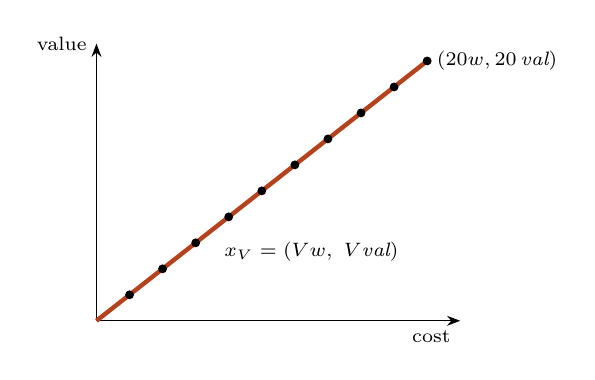
\begin{tikzpicture}[x=4.2mm,y=2.2mm]
  \draw[-{Stealth}] (0,0) -- (11,0) node[below left]{\scriptsize cost};
  \draw[-{Stealth}] (0,0) -- (0,16) node[left]{\scriptsize value};
  \draw[ultra thick, new] (0,0) -- (10,15);
  \foreach \v in {1,...,10} \fill (\v,1.5*\v) circle (1.6pt);
  \node[right, font=\scriptsize] at (10,15) {$(20w, 20\,\textit{val})$};
  \node[font=\scriptsize] at (6.5,4) {$x_V = (Vw,\ V\textit{val})$};
\end{tikzpicture}
\end{column}
\begin{column}{.48\textwidth}
\textbf{Knapsack class}: the options $x_V$ all lie on one line through $O$ (same ratio $\textit{val}/w$).
The upper hull is \textbf{one segment} $O \to x_{20}$: item $X$ with \textbf{0..20 copies}, so
(c) gives exactly the LP, $1\,273\,508 < \text{MIN}$.\\[1mm]
If $x_{20}$ becomes false, the segment just gets shorter ($O\to x_{19}$): its slope does not change.
\end{column}
\end{columns}
\vspace{2mm}
\begin{itemize}\setlength\itemsep{2pt}
\item \textbf{amosum}: a group with only an AMO and no capacity ($R = \infty$). Dantzig takes every segment, so
  $UB = $ the top of the hull $= \max_i p_i$ over the undefined options. That is \textbf{amosum's mps}.
  (Implementation: such groups keep amosum's $O(1)$ max and need no hull.)
\item \textbf{Flat item} (in no AMO): a class with one option, so one segment $O \to (v, w)$; this is case (b).
\item The toy example: $\{a\}$ alone, and $\{b\},\{c\}$ in the capacity 2: $UB = 5 + 3 + \frac12\cdot 2 = 9$; with $a$ false, $4 < 5$.
\end{itemize}
\end{frame}

\begin{frame}{The hull during search}
\footnotesize
\begin{columns}[T]
\begin{column}{.36\textwidth}
\centering
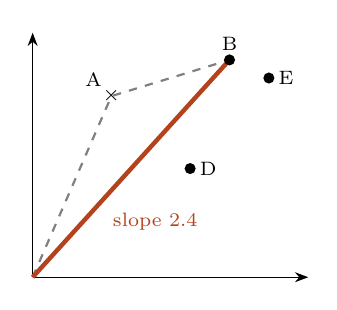
\begin{tikzpicture}[x=5mm,y=2.3mm]
  \draw[-{Stealth}] (0,0) -- (7,0);
  \draw[-{Stealth}] (0,0) -- (0,13.5);
  \draw[thick, gray, dashed] (0,0) -- (2,10) -- (5,12);
  \draw[ultra thick, new] (0,0) -- node[below right, pos=.35]{\scriptsize slope 2.4} (5,12);
  \draw (2,10) node{\scriptsize$\times$} node[above left]{\scriptsize A};
  \foreach \n/\x/\y/\pos in {B/5/12/above, D/4/6/right, E/6/11/right}
     \fill (\x,\y) circle (2pt) node[\pos]{\scriptsize \n};
\end{tikzpicture}\\
\scriptsize $A$ became false
\end{column}
\begin{column}{.62\textwidth}
\begin{itemize}\setlength\itemsep{2pt}
\item \textbf{An option becomes false}: remove its point and recompute the class hull, $O(k)$ for class size $k$.
  Here the new segment $O\to B$ has slope $2.4$, \emph{a slope that did not exist before}.
\item A \textbf{dominated} option ($D$, $E$) becomes false: the hull does not change, so there is nothing to do.
\item \textbf{An option becomes true}: the class is decided. It contributes $p_l$ exactly, uses $c_l$ of $R$, and its
  segments leave the list (the other options become false by the AMO).
\item \textbf{Undo}: the same operations in reverse.
\end{itemize}
\end{column}
\end{columns}
\vspace{1mm}
\begin{block}{Data structure (per capacity group)}\scriptsize
New slopes appear, so a static Fenwick array (fixed order) is not enough. Instead, a \textbf{balanced search tree} (a treap)
holds all current segments keyed by slope, and each node stores the subtree sums $(\sum\Delta c, \sum\Delta p)$.
\begin{itemize}\setlength\itemsep{0pt}
\item critical segment / $UB$: one descent, $O(\log n)$;
\item class update: delete its old segments and insert the new ones, $O(h \log n)$ with $h$ = hull size (1 for Knapsack).
\end{itemize}
\end{block}
\end{frame}

\begin{frame}{Dual view: the price of capacity}
\footnotesize
Let $\lambda$ = the slope of the critical segment (the ``price'' of one unit of capacity). Then
\[
UB \;=\; T \;+\; \lambda R \;+\; \sum_C g_C(\lambda), \qquad
g_C(\lambda) = \max\big(0,\ \max_{i\in C}\,(p_i - \lambda c_i)\big),
\]
where $g_C$ is the best \emph{profit} of class $C$ when capacity costs $\lambda$. This is LP duality: for any
$\lambda \ge 0$ the right-hand side is an upper bound, and it is tight at the critical slope.
\vspace{1mm}
\begin{itemize}\setlength\itemsep{2pt}
\item Example: $\lambda = 3$, $R = 6$: $g_{C_1} = \max(0,\ 10{-}6,\ 12{-}15,\ 6{-}12,\ 11{-}18) = 4$,
  $g_{C_2} = \max(0, 9{-}9, 18{-}18) = 0$, so $UB = 18 + 4 + 0 = 22$. \checkmark
\item \textbf{Option 3} (motivating example) is this formula with $\lambda$ \emph{frozen at the root}, written as one
  \texttt{\#sum}. \textbf{Option 2} (jointsum) re-optimises $\lambda$ at every node.
\item \textbf{Cheap tests} for propagation (next slide) come from this formula: forcing or removing one option changes
  only that class's $g_C$, so the drop has a lower bound that needs no new Dantzig run.
\end{itemize}
\end{frame}

\begin{frame}{Propagation and reasons}
\footnotesize
Slack $s = \text{mps} - K$; $s < 0$ is a conflict. For an undefined option $l$ in class $C$:
\begin{itemize}\setlength\itemsep{2pt}
\item \textbf{$\neg l$} if $UB - UB[l{=}\top] > s$.\\
  Quick test: the drop is $\ge g_C(\lambda) - (p_l - \lambda c_l)$ (the reduced cost). If that is $> s$, propagate.
  Otherwise fix $l$ ($T \mathrel{+}= p_l$, $R \mathrel{-}= c_l$, remove $C$'s segments), take one descent, and restore.\\
  Example: fix $B$: $4 - (12 - 15) = 7$, so $UB[B] \le 15$ (the exact value is 15).
\item \textbf{$l$} if $UB - UB[l{=}\bot] > s$. Only \textbf{hull vertices} can qualify, since removing a dominated option changes nothing.
  Quick test: drop $\ge g_C(\lambda) - g_{C\setminus l}(\lambda)$. Exact: rebuild $C$'s hull without $l$, take one descent, and restore.
\item \textbf{amosum check}: with no capacity, these become \texttt{propagateGeAmo}: ``max must be true'' and ``lighter literals first''.
\end{itemize}
\vspace{1mm}
\textbf{Reason} = the false options that shape the hulls (of the other classes, and of the derived literal's class for
$l$ true) + the true literals that use capacity or decide a class.\\
\textbf{Minimisation} (generalises \texttt{--reason min}): a greedy pass that \emph{restores} each candidate (re-insert the
point, update the hull and the tree), takes $\text{inc} = UB_{\text{new}} - UB_{\text{old}}$, keeps the restore if the
cumulative increment stays $\le s_h$, and rolls everything back at the end. It is exact, so it is sound by construction.
\end{frame}

\begin{frame}{Where jointsum plugs into the pipeline}
\scriptsize
\setlength{\tabcolsep}{3pt}
\renewcommand{\arraystretch}{1.05}
\begin{tabular}{>{\raggedright\arraybackslash}p{15mm}>{\raggedright\arraybackslash}p{33mm}>{\raggedright\arraybackslash}p{92mm}}\toprule
stage & amosum (untouched) & jointsum \\\midrule
syntax & \texttt{\#amosum\{W,T:c[G]\} >= B} & \GEN: \texttt{\#jointsum\{W,T:c\} >= B} / \texttt{<= B}, i.e.\ \texttt{\#sum} syntax without groups\\
parser & \texttt{amosum\_rule} $\to$ \texttt{\_\_group\_\_}\dots & \GEN: grammar rule \texttt{jointsum\_rule}; a transformer method that reuses \texttt{element\_rules}; emits \texttt{\_\_jelement\_\_}, \texttt{\_\_jlb\_\_}/\texttt{\_\_jub\_\_}\\
grounder & \texttt{AmosumGrounder}, \texttt{normalize} & \NEW\ \texttt{JointsumGrounder}: one \texttt{JointsumConstraint} per statement (a tuple counts once); then \textbf{groups and classes are built} from the statements (target / AMO / capacity / nesting)\\
init & \texttt{AmoclingoPropagator} & \NEW\ \texttt{JointclingoPropagator : fiore::PropagatorPBConstraint}, one per target statement\\
propagation & \texttt{AmosumPropagator} & \NEW\ \texttt{JointsumPropagator}: hulls, segment treap, Dantzig, reasons; same fiore template\\
search & \texttt{core/cpp/search} & optimisation: future work\\
command & \texttt{amoclingo}, \texttt{amowasp} & \NEW\ \texttt{jointclingo} (clingo only, C++), in \file{jointsum/jointclingo/}; propagator code in \file{jointsum/core/cpp/jointsum/}; \texttt{amoclingo}/\texttt{amowasp} unchanged\\
tests & \texttt{check\_correctness.py} & oracle: \texttt{\#jointsum} $\to$ \texttt{\#sum} in plain clingo (same answer sets);
  amosum as \texttt{\#jointsum} (target + one \texttt{<= 1} per group) $\equiv$ \texttt{\#amosum}; Knapsack 0056/0096 UNSAT at the root\\\bottomrule
\end{tabular}
\end{frame}

%=====================================================================
\section{Part IV --- jointsum and plain LP}

\begin{frame}{LP in one picture}
\footnotesize
\begin{columns}[T]
\begin{column}{.48\textwidth}
Two items of the toy knapsack, capacity 4:
\[
\begin{aligned}
\max\ & 8x_1 + 9x_2\\
\text{s.t. } & 2x_1 + 3x_2 \le 4\\
& 0 \le x_1, x_2 \le 1
\end{aligned}
\]
\begin{itemize}\setlength\itemsep{2pt}
\item The \textbf{feasible region} (shaded) is a convex polygon, a \emph{polytope} in $n$ dimensions, cut out by the constraints.
\item The objective is a direction (arrow). Push the line $8x_1 + 9x_2 = z$ as far as it goes inside the region.
\item The optimum is always at a \textbf{vertex}: here $(1, \frac23)$ with value $8 + 6 = \mathbf{14}$.
\item Dantzig finds the same point: item 1 whole (ratio 4), then $\frac23$ of item 2 (ratio 3).
\end{itemize}
\end{column}
\begin{column}{.5\textwidth}
\centering
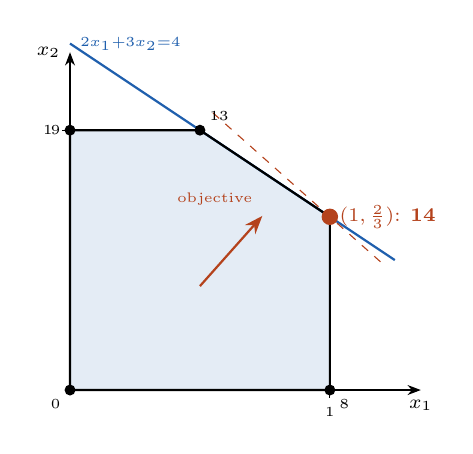
\begin{tikzpicture}[scale=3.3]
  \fill[acc!12] (0,0) -- (1,0) -- (1,0.6667) -- (0.5,1) -- (0,1) -- cycle;
  \draw[-{Stealth}] (0,0) -- (1.35,0) node[below]{\scriptsize $x_1$};
  \draw[-{Stealth}] (0,0) -- (0,1.3) node[left]{\scriptsize $x_2$};
  \draw (1,0) -- (1,-0.03) node[below]{\tiny 1};
  \draw (0,1) -- (-0.03,1) node[left]{\tiny 1};
  \draw[thick, acc] (0,1.3333) node[right]{\tiny $2x_1{+}3x_2{=}4$} -- (1.25,0.5);
  \draw[thick] (0,0) -- (1,0) -- (1,0.6667) -- (0.5,1) -- (0,1) -- cycle;
  \draw[dashed, new] (0.55,1.0667) -- (1.2,0.4889);
  \draw[-{Stealth}, new, thick] (0.5,0.4) -- (0.74,0.67) node[above left]{\tiny objective};
  \foreach \x/\y/\v/\p in {0/0/0/below left, 1/0/8/below right, 0.5/1/13/above right, 0/1/9/left}
     \fill (\x,\y) circle (0.6pt) node[\p]{\tiny \v};
  \fill[new] (1,0.6667) circle (0.9pt) node[right]{\scriptsize $(1,\frac23)$: \textbf{14}};
\end{tikzpicture}
\\[1mm]\scriptsize vertices with their value $8x_1+9x_2$
\end{column}
\end{columns}
\end{frame}

\begin{frame}{Finding a feasible point (Phase I), and proving there is none}
\footnotesize
\textbf{Problem}: given $Ax \le b$, $x \ge 0$, find \emph{some} $x$, or prove that none exists.\\[1mm]
\textbf{Trick}: turn it into an optimisation problem that \emph{has} an obvious feasible start. Add one extra variable $t \ge 0$
that relaxes every row:
\[
\min\ t \quad\text{s.t.}\quad Ax - t\,\mathbf{1} \le b,\quad x \ge 0,\ t \ge 0 .
\]
\begin{itemize}\setlength\itemsep{2pt}
\item Start: $x = 0$, $t = \max(0, -\min_i b_i)$ is feasible, so we can begin anywhere.
\item Solve it like any LP (next slide). Then \textbf{optimum $t = 0$} means the returned $x$ is feasible for the original
  problem, and \textbf{optimum $t > 0$} means the original problem is \textbf{infeasible}.
\end{itemize}
\vspace{1mm}
\begin{block}{Certificate of infeasibility (Farkas' lemma)}
$Ax \le b,\ x\ge 0$ is infeasible $\iff$ there are multipliers $y \ge 0$ with $y^{\top}\!A \ge 0$ and $y^{\top} b < 0$:
a non-negative combination of the rows that reads ``$0 \le$ something negative''.\\[1mm]
\textbf{We have already seen one!} In Option 3, $(V)$ and $(W)$ with multiplier $\lambda = 2$ combined into
``$7 \ge \text{left side} \ge 8$''. The LP solver returns such a $y$ (the dual solution), and an LP propagator turns it
into the reason of the conflict.
\end{block}
\end{frame}

\begin{frame}{How an LP is solved: three algorithms}
\footnotesize
\renewcommand{\arraystretch}{1.25}
\begin{tabular}{>{\raggedright\arraybackslash}p{24mm}>{\raggedright\arraybackslash}p{62mm}>{\raggedright\arraybackslash}p{48mm}}\toprule
algorithm & idea & running time\\\midrule
\textbf{Simplex}\newline(Dantzig, 1947)
  & Walk from vertex to adjacent vertex, always improving the objective (a \emph{pivot}), until no neighbour is better.
  & \textbf{Exponential} in the worst case (Klee--Minty cubes, 1972), but fast in practice and polynomial in the smoothed
    sense (Spielman--Teng, 2004).\\
\textbf{Ellipsoid}\newline(Khachiyan, 1979)
  & Keep an ellipsoid that contains the feasible region; test its centre; if it violates a row, cut the ellipsoid in half
    and take a smaller one around the good half. It shrinks by a fixed factor per step.
  & \textbf{Polynomial}: $O(n^2 L)$ iterations, $L$ = bits of the input. The first proof that LP $\in$ P; slow in practice.\\
\textbf{Interior point}\newline(Karmarkar, 1984)
  & Move through the \emph{inside} of the polytope along the ``central path'' (a barrier keeps you away from the walls),
    with Newton steps toward the optimum.
  & \textbf{Polynomial}: $O(\sqrt{n}\,L)$ iterations, each one solving a linear system. Fast in practice too.\\\bottomrule
\end{tabular}

\end{frame}

\begin{frame}{Polynomial is not the same as cheap enough per node}
\footnotesize
\begin{itemize}\setlength\itemsep{2pt}
\item \textbf{Phase I + any polynomial algorithm} gives a feasible point (or a Farkas certificate) in polynomial time.
  With integrality ($x \in \{0,1\}$) the same question becomes NP-hard, which is why the LP is used as a \emph{relaxation}.
\item \textbf{Inside a CDCL solver} (clingo[LP], metaprop) the dual simplex is used anyway: after a new bound it restarts from the
  previous optimal basis (\emph{warm start}), usually with a few pivots. Each pivot touches the whole tableau, $O(m \cdot n)$.
\end{itemize}
\vspace{1mm}
\begin{center}\scriptsize
\begin{tabular}{>{\raggedright\arraybackslash}p{30mm}>{\raggedright\arraybackslash}p{56mm}>{\raggedright\arraybackslash}p{52mm}}\toprule
 & general LP & \texttt{\#jointsum} group\\\midrule
problem & any $Ax \le b$ & 1 capacity + AMO classes (MCKP LP)\\
from scratch & polynomial (interior point), simplex in practice & sort the hull segments: $O(n \log n)$\\
after one literal changes & warm-started dual simplex: some pivots, $O(m n)$ each & update a hull and the treap: $O(h \log n)$\\
after backtracking & restore or repair the basis & undo the same updates\\
arithmetic & floating point, with tolerances & exact integers, $\lfloor\cdot\rfloor$\\\bottomrule
\end{tabular}
\end{center}
\vspace{2mm}
The point of \texttt{\#jointsum} is not a better complexity class. Both are polynomial. Its structure (one resource per group,
classes with concave hulls) lets the LP optimum be read off \textbf{greedily} and updated \textbf{incrementally}, so it can be used
\textbf{at every propagation}, like an ordinary aggregate.
\end{frame}

\begin{frame}{\texttt{\#jointsum} vs a plain LP propagator: what we gain}
\footnotesize
On the structures it covers (one capacity group with nested AMO classes) the bound is \textbf{the same} as the LP of that
sub-problem: on 0096 both are $1\,273\,508$. The gain is everything \emph{around} the bound:
\begin{enumerate}\setlength\itemsep{2pt}
\item \textbf{Cost per node}: $O(\log n)$ per change and trivial undo, against re-optimisation and basis restore. So it runs
  at every propagation, where LP propagators often run less often or only check feasibility.
\item \textbf{Real propagation}: for each undefined literal it decides exactly whether it is forced true or false (an $O(1)$
  reduced-cost filter, then one descent). An LP does this exactly only by \emph{probing} (one LP per literal); cheaply, it only
  has reduced-cost fixing, which is just our quick test.
\item \textbf{Small explanations}: the LP explains a conflict by its Farkas certificate, i.e.\ all the literals behind the
  active bounds, large and never minimised. \texttt{\#jointsum} builds the reason from the hulls and minimises it greedily.
  Shorter learned clauses mean better learning and backjumping.
\item \textbf{Exact arithmetic}: integers and floors, so no tolerances and no risk of a missed or wrong propagation.
\item \textbf{A bit of integrality}: each group is floored separately ($\sum\lfloor\cdot\rfloor \le \lfloor\sum\cdot\rfloor$),
  and small groups can use an exact DP instead of the LP.
\item \textbf{It fits the system}: the encoding as written, no external solver, no variables or rows linking LP variables to
  atoms, one propagator per thread as in amosum.
\end{enumerate}
\end{frame}

\begin{frame}{\texttt{\#jointsum} vs a plain LP propagator: where the LP is stronger}
\footnotesize
\begin{itemize}\setlength\itemsep{4pt}
\item \textbf{Several resources on the same literals} (multi-dimensional knapsack): the LP combines all of them, each with
  its own multiplier; \texttt{\#jointsum} uses one price $\lambda$ per group.
\item \textbf{Overlapping side constraints without nesting}: the LP treats them jointly; v1 assigns each literal to one side
  constraint (weight splitting is future work).
\item \textbf{Groups restricted by \texttt{<=} and \texttt{>=} at once}: a general LP, with no greedy solution.
\item \textbf{Long chains across many constraints}: the LP reasons over all of them at once; \texttt{\#jointsum} connects
  them only through propagation on assigned literals.
\end{itemize}
\vspace{3mm}
\begin{block}{About the motivating case}
metaprop's LP missed UNSAT on Knapsack because the weight constraint was \emph{not in the LP}, not because LP is too weak.
With the weight constraint included, the LP finds the same bound. The case for \texttt{\#jointsum} is therefore:
\textbf{LP strength on the structure it covers, at the cost of an incremental update, with per-literal propagation and
short reasons}, which is what makes the bound useful at every node of a CDCL search.
\end{block}
\end{frame}

%=====================================================================
\section{Part V --- decisions}

\begin{frame}{Decisions}
\footnotesize
\begin{itemize}\setlength\itemsep{3pt}
\item \textbf{Syntax}: \texttt{\#jointsum\{ W,T : cond ; ... \} >= B} and \texttt{<= B}, i.e.\ classical \texttt{\#sum} syntax with no groups.
\item \textbf{Scope}: only \texttt{\#jointsum} statements; every statement is both a target and a side constraint.
\item \textbf{Bound}: nested classes (MCKP, hulls) in v1; \texttt{>=} and \texttt{<=} together (mirror images).
\item \textbf{Code}: C++ only. Code may be shared with amosum as long as amosum's behaviour does not change. Python only
  changes where the commands need it (the \texttt{jointclingo} wrapper, the parser).
\item \textbf{Layout}: \file{jointsum/jointclingo/\{\_\_main\_\_.py, cpp/\}} and \file{jointsum/core/cpp/jointsum/}; \file{amosum/}
  (with \texttt{ijcai\_version}, \texttt{amoclingo}, \texttt{amowasp}, the Python version) is unchanged.
\item \textbf{Future work}: optimisation (\texttt{\#jointmaximize}); weight splitting for overlaps that are not nested;
  groups restricted by $\le$ and $\ge$ at once (general LP).
\end{itemize}
\vspace{2mm}
\centering\textcolor{new}{Nothing is implemented yet.}
\end{frame}

\end{document}
